\chapter{Introduction}
\label{chapter:intro}
\pagestyle{mainmatter}
\pagenumbering{arabic}

\epigraph{\small\itshape ``Progress in science depends on new techniques, new discoveries and new ideas, probably in that order.''}{\small\textit{---Sidney Brenner}}

Understanding the human brain is one of the most significant challenges of the 21st century. The human brain is arguably one of the most complex  organs of the human body, which performs a wide range of cognitive functions: from visual recognition to language understanding, speech, social interaction, and executive control. Pathologies of the brain are perhaps on of the biggest challenges for western medicine today. Medical interventions and drugs for major infectious diseases are available today, and individuals can expect to live up to the mid 80s and even into their 90s. Yet, we still do not have a good grasp over most mental pathologies: Parkinson's, Alzheimer's, dementia, epilepsy to name a few. This is despite the fact that someone today who lives into their mid 80s has a 50\% chance of contracting Alzheimer's~\citep{alzheimer20162016}.

Our current understanding of the brain is a result of decades of concerted efforts across multiple disciplines ranging from molecular biology, genetics, physiology, cognitive and behavioral neuroscience, to statistics, computer science, and data science. A relatively new subfield here is brain imaging, also known as neuroimaging. Brain imaging refer to a set of technologies where a snapshot of the brain is taken to measure either the anatomy or various aspects of function. The grand vision of is to be deploy them in hospitals to help diagnosis, in surgeries, in \acp{BCI}, or in research for neuroscientists to better understand the brain. In this thesis, we will focus our attention on measuring the electric and/or corresponding magnetic field from the brain, using electroencephalography, magnetoencephalography, and local field potentials. These methods have the property of possessing a high temporal resolution, which is particularly useful for extracting the temporal dynamics of brain signals.

In the following sections, I will describe the context surrounding the thesis. After a brief introduction to the field of electrophysiology, I will delve into how the field has been shaped in recent years by the reproducibility crisis, and how data sharing is going to help alleviate this problem to a large extent. However, the rise of data sharing and large sample sizes makes it difficult to still rely on manual data analysis which does not scale and is not reproducible. To cope with this challenge, we must start relying on automated and data-driven methods for discovering new effects.
 
%\section{Modern brain imaging}
%Brain imaging tools today can be placed along three axes: their temporal resolution, their spatial resolution, and the level to which they are invasive.

\clearpage

\section{Electrophysiology}

\begin{figure}[htb]
\begin{center}
   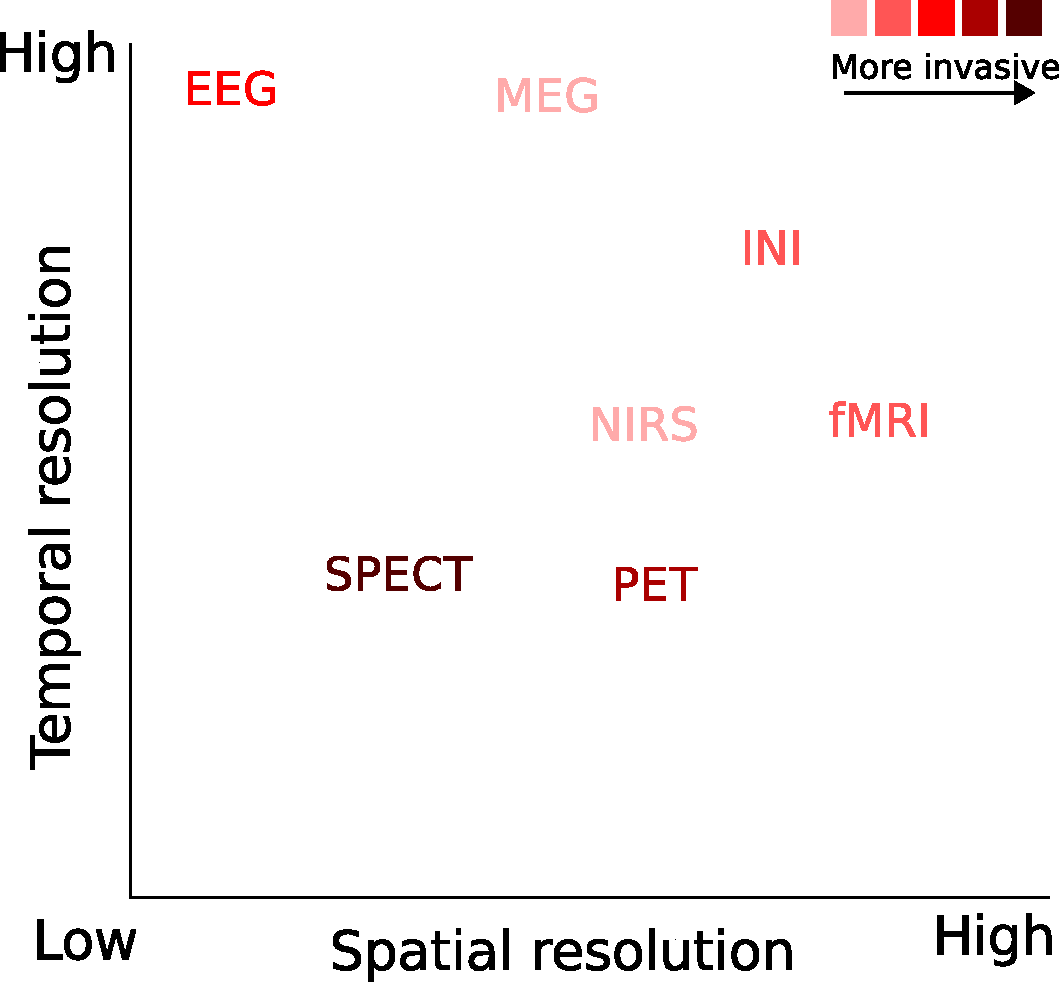
\includegraphics[width=0.5\linewidth]{figures/neuroimaging_methods.pdf}
\end{center}
   \caption[Various neuroimaging methods differ in terms of the information they measure.]{Various neuroimaging methods differ in terms of the information they measure. MEG=magnetoencephalography, EEG=electroencephalography, NIRS=near-infrared spectroscopy, PET=positron emission tomography, SPECT=single photon emission tomography, and INI=Inverse imaging, a method to speed up acquisition of fMRI images, ECoG=Electrocorticography, LFP=Local Field Potential.}
   \label{fig:neuroimaging_methods}
\end{figure}

The study of electrical properties of the biological cells and tissues is known as electrophysiology. Biological tissues have electrical properties due to the presence of ions. Just as we can measure voltages in electrical appliances, it is possible also to measure these voltages on living tissues. These modalities have the advantage of directly measuring the brain activity, as opposed to an indirect measure, which is for example the case in \ac{fMRI}.
Brain imaging techniques are characterized by their temporal and spatial resolution, \textit{i.e.,} the time scale at which it can measure brain activity, and also the accuracy of localizing the source of the activity. Figure~\ref{fig:neuroimaging_methods} summarizes different neuroimaging methods with respect to their temporal and spatial resolution. In the case of \ac{fMRI}, as it measures the blood flow which is a response to neural activity and slowly changing, its temporal resolution cannot be high. 

There are a number of modalities to measure the electrical potentials, the most well-known being perhaps \ac{ECG} which is used to measure the heart beats. However, in our work, we will focus on only three which are relevant for studying the brain.

\paragraph{Electroencephalography: } \Ac{EEG} is a portable and non-invasive measurement modality that is frequently used in the context of \acp{BCI}. In electroencephalography, an array of electrodes on an \ac{EEG} cap are placed on the scalp to measure the voltages with respect to a reference electrode. The voltage it measure is not the result of a single neuron but instead a summed potential of populations of thousands of neurons. It has a high temporal resolution (in the order of \emph{ms}), however the spatial resolution is not so high as the skull smears the signal.

\paragraph{Magnetoencephalography: } Any electric current is associated with magnetic fields as a consequence of Maxwell's theory. Therefore, the brain generates tiny magnetic fields which are wrap around the currents according to Maxwell's right hand thumb rule. The flux is tiny ($\sim10^{-12}T$) compared to the earth's magnetic field ($10^{-4}T$), and to measure this one would need very sensitive electronics and heavy noise cancellation. The measurement itself is done done in a shielded magnetic room made of three layers of metals. The sensors are superconducting coils which capture the magnetic flux. They are immersed in liquid helium cooled to very low temperatures, so as to lower any loss in signal due to resistance. A typical device contains two types of sensors: gradiometers and magnetometers. While the magnetometer measures the absolute magnitude of magnetic field, the gradiometer measures derivative of the field. It is therefore less sensitive to external noise [\mainak{check}]. \ac{MEG} has the advantage that the skull does not deteriorate the signal quality.

\paragraph{Local Field Potential (LFP)}
The Local Field Potential is an invasive method that measures the electrical potential in the extracellular space of the brain tissue. In contrast to \ac{EEG}, LFP are recorded in depth, from within the cortical tissue and can therefore measure more localized populations of neurons.

\section{The reproducibility crisis}

Even though thousands of papers are published every year about different aspects of the brain, our understanding of this complex organ has not scaled in proportion. A large part of the reason has been attributed to what is known as the reproducibility crisis~\citep{ioannidis2005most, simmons2011false, button2013power}. %Replication is closely related to the concept of reproducibility which refers to the idea that an experiment produces the same result when performed again under the same conditions. Replication is a stronger condition as it requires similar results or identical conclusion even if there are some minor variations in the experimental procedures. 
Progress in science rests on reproducible experiments. Reproducibility refers to the fact that the findings of an experiment can be regenerated if the code, data, and related software was provided to an independent . In many fields, however, a large fraction of experiments cannot be reproduced. In psychology, for instance, it was estimated that over half of the papers were not reproducible~\citep{open2015estimating}, and even those which could be reproduced tended to have a weaker effect size compared to the original study. 

The reasons for unreproducible results can be many~\citep{baker20161}, some being: 1) confirmation bias, the tendency to selectively report only experiments that conform to the researcher's pre-existing beliefs, 2) ``p-hacking''~\citep{simmons2011false}, or the tendency to try multiple hypothesis to get a positive result, 3) publication bias or the absence of incentives to publish negative results~\citep{rosenthal1979file}, and 4) pressure to publish. There are now an accepted set of recommendations to counter many of these issues: 1) pre-registering research plans to avoid confirmation bias and even report negative results, 2) correct for multiple comparisons, the most conservative method being the Bonferroni correction~\citep{dunn1961multiple}. 

Brain imaging has its own set of issues which can be linked to reproducibility crisis: 

% vul2009puzzlingly
% yendiki2014spurious

\begin{itemize}[noitemsep,partopsep=0pt]
\item \textbf{Power failure:} This is arguably one of the central issues in the reproducibility crisis today and has received by far the most attention. The statistical power of a study refers to the likelihood of discovering an effect of interest, given the sample size. Small sample sizes translate into underpowered studies which means that the chance of a false discovery is high. In order to discover the effect of interest, the study must be appropriately powered.
\item \textbf{Multiple comparison:} This is essentially a manifestation of ``p hacking'' that is a result of of the large number of voxels or time points in neuroimaging. For instance, in the famous dead salmon study~\citep{bennett2009neural}, a significant effect was found even if none was expected simply because the hypothesis testing (comparisons) were done over each voxel.
\item \textbf{Differences in software versions:} Changing software versions can lead to different results. For instance in the case of Freesurfer software, differences in volume were found in the range of $8.8\% \pm 6.6\%$ was found~\citep{gronenschild2012effects}.
\item \textbf{Complex pipelines:} Neuroimaging pipelines involve a number of choices at each processing stage, and there isn't currently a consensus on how to choose the right pipeline. Often, these methodological choices are not even documented. It is estimated that almost every new study has its own unique pipeline~\citep{Carp2012289}.
\item \textbf{Confounds:} There are several methodological confounds such as head movements~\citep{yendiki2014spurious}, anatomy differences, and changes in breathing rate and depth, which can lead to spurious correlations.
\end{itemize}

In Chapter~\ref{chapter:group_study} of the thesis, we will provide concrete guidelines on how to build processing pipelines for \ac{MEG}/\ac{EEG} data. Our contribution will touch upon the issue of complex pipelines, multiple comparison, and differences in software versions in the context of \ac{MEG}/\ac{EEG}. The issue of power failure can be alleviated through data sharing as I will discuss in the next section.

\section{Data sharing}
\label{sec:intro_datasharing}
Power failure is essentially a consequence of small datasets. In today's collaborative and data-driven scientific environment, data sharing is useful not only from the perspective of reproducibility but also to build datasets with large sample sizes. With large datasets, it would be possible to tease apart even subtle effects~\citep{smith2017statistical} that were not possible with smaller datasets. Data sharing is beneficial not just from the perspective of replication but also from an economic perspective. Rather than collect new data for every new hypothesis, researchers can now reuse known data for answering their hypotheses.

The benefits of data sharing can be traced back to Newton and his theory of gravitation~\citep{pointofview2013}. Before Newton had developed his theory, another English astronomer, John Flamsteed had been appointed by the king to observe the stars and produce accurate charts for navigation in the seas. Over a period of 40 years, Flamsteed created a detailed catalogue that tripled the number of entries in the previously used sky atlas. When the great comet of 1680 appeared in the sky twice in close succession, Flamsteed used his data to postulate that it was not two comets but in fact the same comet which first went towards the sun and then turned away from it. Newton initially opposed this theory, but later changed his mind as he gained access to Flamsteed's unpublished catalogue. The comet had indeed turned out to be an important benchmark for Newton's theory of gravitation.

It is hard to imagine in this day and age that a theory as fundamental as the laws of gravitation could have been data driven. Data sharing is fundamental not only to reproducible science, but also it forms the cornerstone for learning stronger models and benchmarking new algorithms. Consequently, in machine learning, recent breakthroughs have been powered by the increase in data sharing and computation. This includes the recent resurgence of deep learning~\citep{deng2009imagenet}, Q learning~\citep{watkins1992q, bellemare2013arcade}, natural language processing for language translation~\citep{halevy2009unreasonable}, speech recognition~\citep{paul1992design}, and even the mixture of experts model~\citep{jacobs1991adaptive} for IBM Watson~\citep{ferrucci2010building}. The maxim, ``more data beats a cleverer algorithm''~\citep{domingos2012few} has held up remarkably well across disciplines and over the ages.

Of course, neuroscientists are beginning to realize the importance of sharing data. In recent times, neural data has started being shared through international consortiums~\citep{van2013wu, ollier2005uk} and data repositories~\citep{poldrack2013toward, gorgolewski2015neurovault}. While in the case of Newton, he gained access to the catalogue without permission, today it is possible to publish dataset papers in targeted journals so as to assign the credit where it is due. Yet, there is an unaddressed gap in terms of the ideal of data sharing and the practice of data sharing. Neuroimaging experiments are often very complicated, and it is not enough to share simply the data, but also the metadata and information regarding the experimental protocols in a well-structured format. In the absence of this information, shared data is not \emph{reusable} in the same way that uncommented and spaghetti code is not useful even if shared publicly. There isn't an accepted consensus in the community on the practices of sharing data and there is a need to establish a standard. In Chapter~\ref{chapter:group_study}, we will present a new standard known as the \ac{BIDS}, which is intended to address this gap. It is a collaborative effort between software developers and neuroscientists across various laboratories to establish a consensus on the standards and build tools to facilitate adoption of the standard.

\section{Automation}

Back in 2014, Nature published a bold article~\citep{hayden2014automated} which described a vision for the future of science: ``solving the problem of bringing McDonald's-like efficiency to scientists''. This would in turn lead to cheaper, more efficient and reliable research. While it goes on to describe many biology labs which are automating experiments, the benefits of automation in the neuroimaging community are yet to be widely recognized. Automation not only saves time but also makes the research more reproducible, as was noted in a recent guide to improve the transparency and reproducibility of neuroimaging research~\citep{gorgolewski2016practical}. The authors point out that manual work may seem easy at first, if the analysis has to be performed only once. However, this is not always the case as ``quite often in the course of a project, parameters are modified, subjects are changed, and processing steps need to be rerun. This is a situation in which having a set of scripts that can perform all of the processing steps automatically instead of relying on manual interventions can really pay off.'' As large datasets become more common in neuroimaging, automation will indeed become a necessity rather than a luxury.

In neuroimaging, there are in fact several avenues for automation:
\begin{itemize}[noitemsep,nolistsep,nosep]
\item \textbf{Reducing interactivity:} While interactive graphical user interfaces are excellent tools for browsing the data, they fall short when it comes to scaling the analysis, which is necessary for a sufficiently powered study. 

\item \textbf{Parameter tuning:} Most algorithms, although scripted, still require hyperparameters to be tuned. These hyperparameters could be the number of ICA components to choose or the regularization parameters, and can vary for each subject.
%This could be the number of trials to perform in an experiment, the number of components to select in a \ac{PCA} decomposition, or the regularization parameter in inverse solvers.
\item \textbf{Annotation and labeling:} A large fraction of neuroimaging data that is available is unlabeled or at best weakly labeled. This is because expert annotations are expensive, and cannot be crowdsourced. Automated tools based on unsupervised learning can play a major role in this regard.
\item \textbf{Quality control:} Currently, quality control is performed manually by inspecting the data to spot outliers. While data inspection cannot be overlooked, it can be performed more efficiently through automated documentation of data analysis and log reports such as the Jupyter notebook and the MNE web report. At the same time, advanced statistical trend analyses as in the Automated Statistician project~\citep{duvenaud2013structure} can be used for creating summaries.
\end{itemize}

There have been some steps taken in this direction, most notably the Neurosynth platform~\citep{yarkoni2011large} which facilitates large-scale meta analysis to integrate activations maps across studies using machine learning. On the software side, the Freesurfer software package~\citep{dale-fischl-etal:99, fischl-serena-etal:99} provides a \code{recon-all} command that performs cortical segmentation automatically without any human intervention. In MNE, this philosophy is now being adopted~\citep{engemann2015automated_new} starting with automated covariance estimation.

In this thesis, we will consider an algorithm that automatically annotates artifacts in the data~\citep{jas2016automated, jas2017autoreject}. This is a first step that any \ac{MEG}/\ac{EEG} processing pipeline has to go through but it is often done manually. A reason for this is that existing algorithms are not designed to be \emph{transparent}. Since for most scientists, the key to new insights is an artifact-free dataset, they would rather spend extra effort in doing this manually rather than depend on a generic algorithm which is difficult to interpret. %However, this is problematic as it can lead to a selection bias: they might end up rejecting data segments which helps them confirm their hypothesis. 
Merely based on anecdotal reports, this process can take up to a week even for a moderately sized study of 10--20 subjects.

This is what led us to propose \emph{autoreject}, which we describe in Chapter~\ref{chapter:autoreject}. It is an algorithm which can be used to mark bad segments of the data. The key insight is that, often certain sensors in the device are intermittently corrupted rather than continuously. We validate our algorithm against 3 benchmarks on the \ac{HCP} dataset~\citep{larson2013adding} which is manually annotated with bad segments. In the process, our work also represents one of the first attempts at reanalyzing the MEG component of the HCP dataset.

\section{Representation learning for data-driven discovery}
In the last 100 years since the invention of \ac{EEG}, scientists have discovered several different brain oscillation patterns such as alpha waves, K-complexes, and mu rhythms. The oscillations and interactions between them have served as biomarkers for different brain functions and pathologies. Alpha waves have been implicated in attention, K-complexes in sleep, and mu rhythm in motor activity. 

Considering the complexity of the human brain, clearly these waveforms represent only a fraction of the cognitive functions that the brain may perform. As a result of the wealth of data now available through the data sharing movement described in Section~\ref{sec:intro_datasharing}, the future neuroscientist will be able to mine such waveforms from large datasets. Imagine if neuroscientists had at their disposal a tool similar to Google Photos\footnote{\url{https://photos.google.com/}}. In the same way that Google Photos can automatically find faces and group photos, such tools will be able to find prototypical oscillations and cluster the data using them. Clicking on any of these waveforms would retrieve the data associated with them.

\begin{figure}[htb]
\begin{center}
   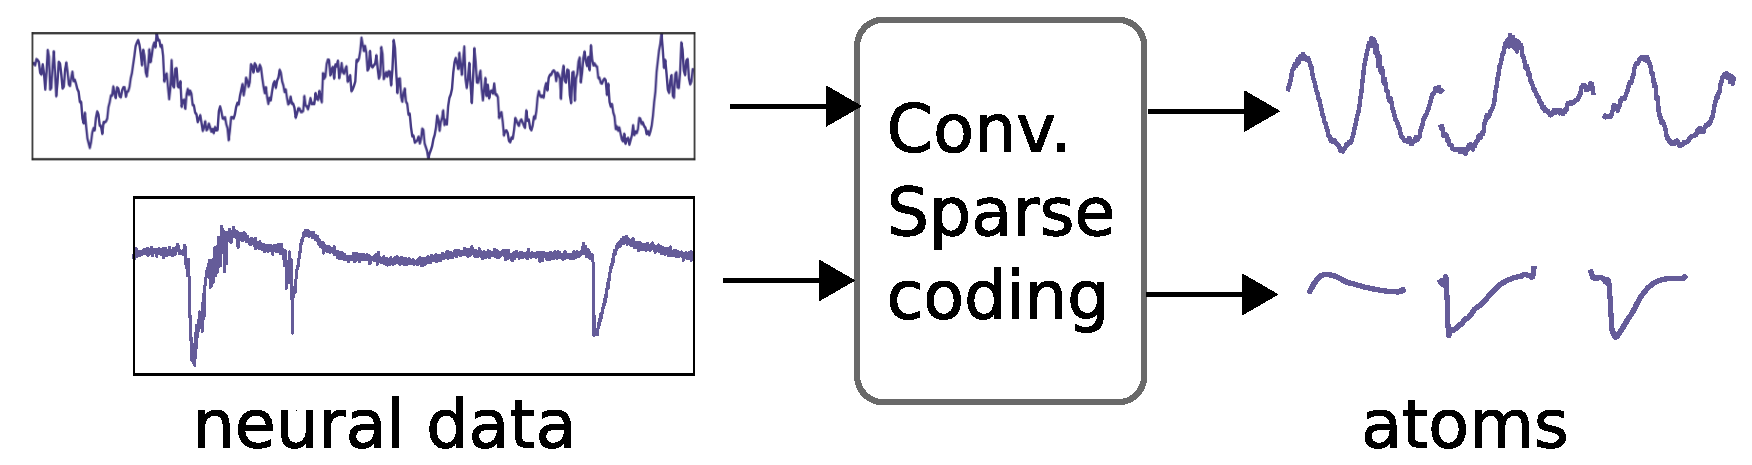
\includegraphics[width=0.7\linewidth]{figures/schema.pdf}
\end{center}
   \caption[Convolutional sparse coding]{An illustration of how Convolutional sparse coding can be used to automatically mine prototypical waveforms}
   \label{fig:neuroimaging_methods}
\end{figure}

However, photos are inherently different from neural data. First, neural data can be buried in noise and corrupted by high amplitude artifacts. Second, images are labelled owing to crowdsourced data as in the case of  Imagenet~\citep{deng2009imagenet}, but neural data is not. 
Expert annotations in the case of neural data are not easily available.
Finally, it is spatiotemporal data with different dynamics than the 3D world that photos capture. This is where \ac{CSC} can play a role by extracting prototypical features from the data. It is an unsupervised algorithm from computer vision, which can learn shift-invariant dictionaries of prototypical waveforms (atoms) from the data using the convolution operations. For a more comprehensive background on \ac{CSC}, the reader may read Section~\ref{sec:background_dict_learning} later in this chapter.

\ac{CSC} algorithms do not approximate the signal using Fourier (or sinusoidal) basis. While this is the conventional technique for extracting signals buried in noise, the approximation can degrade the shape of the signal, which can be a biomarker in many clinical diseases~\citep{cole2017brain}. As an example, a square wave would need an infinite series of sinusoids for a good approximation. Of course, transients can be better approximated using wavelets but it is clearly not sufficient for other shapes of data. Rather than fix the basis to be Fourier or wavelet, the \ac{CSC} approach is to learn \emph{both} the basis and the coefficients.

In our work presented in Chapter~\ref{chapter:alphacsc}, we extend conventional \ac{CSC} algorithms for heavy-tailed noise. We reformulate the optimization problem as a \ac{MAP} inference with an alpha-stable distribution to replace the reconstruction loss. Our results show that this kind of algorithm is robust to the presence of artifacts and can be used to uncover temporal structures from neural signals, even those involving nested oscillations.

\clearpage
\section{Background}

Here, we will introduce some basic linear algebra, optimization, and machine learning concepts that will be useful particularly in Chapters~\ref{chapter:autoreject} and \ref{chapter:alphacsc}.

\subsection{Norms}
Informally speaking, a norm is used to measure the length or size of a vector. It must also satisfy some properties, but it will not be of concern for us in this thesis. It is sufficient to know the mathematical expression, how it behaves, and the physical property that it captures.
\theoremstyle{definition}
\newtheorem{definition}{Definition}[chapter]

\begin{definition}{($\ell_p$ norm.)}
For $1 \leq p < \infty$, the $\ell_p$ norm of a vector $x$ is defined by:
\begin{equation}
\|x\|_p = \Big(\sum_n \ \lvert x_n \rvert^p \Big)^{1/p}
\end{equation}
\end{definition}
%
\begin{definition}{($\ell_\infty$ norm.)}
The $\ell_\infty$ norm of a vector $x$ is defined by:
\begin{equation}
\|x\|_{\infty} = \sup_n \ \lvert x_n \rvert
\end{equation}
\label{def:norm}
\end{definition}
As we are taking the supremum, this norm is sensitive to large values in the vector, which is needed for measuring artifacts.
%
\begin{definition}{(Frobenius norm.)}
The Frobenius norm of a real-valued matrix $A$ is defined by:
\begin{equation}
\|A\|_{\mathrm{Fro}} = \| \mathrm{vec}(A) \|_2 = \sqrt{\mathrm{trace}(AA^\top)}
\end{equation}
%
The Frobenius norm is a matrix norm that is simply the $\ell_2$ vector norm of the vectorized matrix $\mathrm{vec}(A)$.

\end{definition}

\subsection{Cross validation}

Cross validation is a statistical technique to estimate how well a predictive model will \emph{generalize} to unseen data. This is normally done by partitioning the data into two and learning the model from one part (typically the larger one) and validating it on the other. These two parts are known as the \emph{training} and the \emph{validation} sets respectively. In order to get reliable estimates of the model performance, this procedure is repeated multiple times and the results are averaged.

Depending on the data, different types of partitioning schemes are preferred. In \emph{K-fold} cross validation, the data is divided into $K$ equal parts (with or without shuffling the samples), where $K - 1$ parts are used for training and the $K$th part is used for validation. In a \emph{stratified} cross-validation scheme, the partitions are done such that each partition has roughly equal number of samples from each class.

\paragraph{Grid search: } When cross validation is used for selecting the best model by exhaustively searching over all possible parameters that the model can admit, it is known as grid search.

\paragraph{Random search: } Sometimes grid search is too slow, and it is better to try parameters sampled randomly without a considerable loss in performance. This is known as random search.

\paragraph{Nested cross validation: } When cross validation has been used for finding the best model, a separate unseen partition, known as the \emph{test} set, is needed to assess the generalization power of the best model. The test set must be different from all the data that was seen so far, including \emph{both} the training and the validation sets. This is the reason a nested cross-validation scheme is necessary where in each outer loop, the best model is found, and its performance is computed.

\subsection{Bayesian optimization}


\begin{figure}[htb]
\begin{center}
   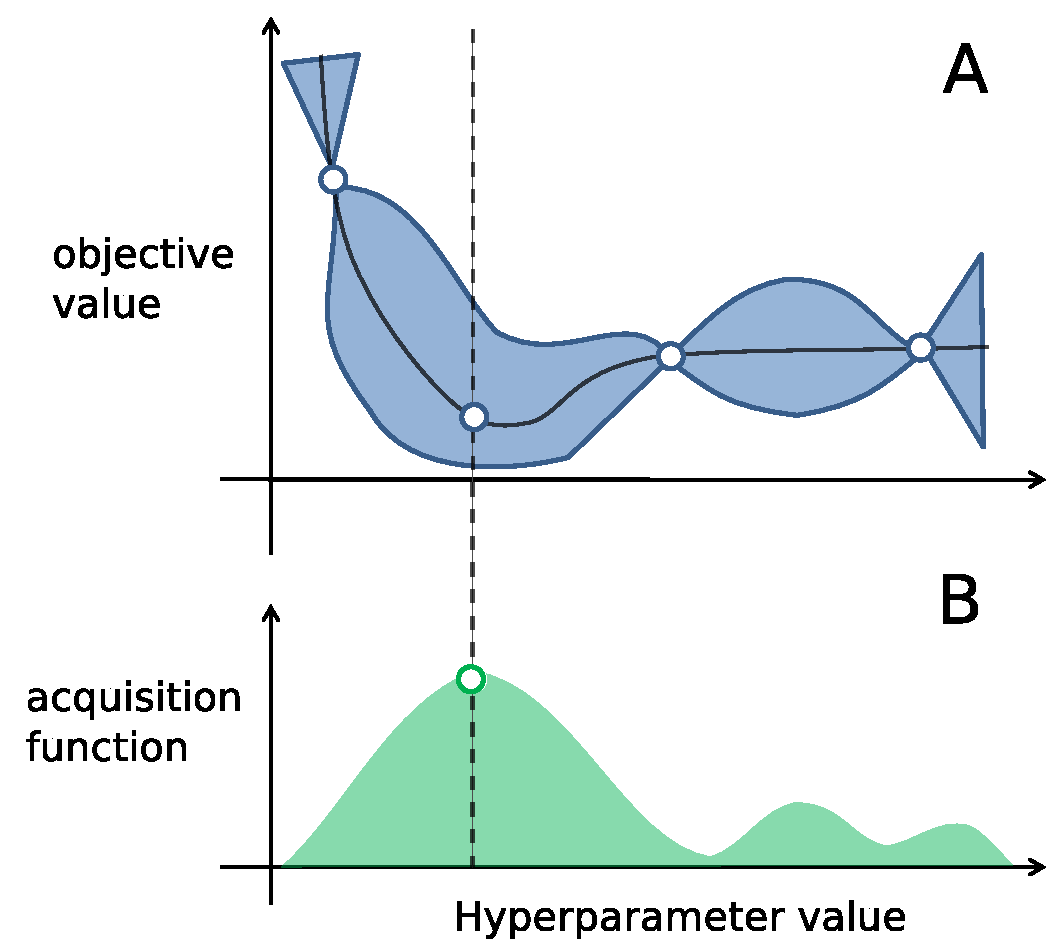
\includegraphics[width=0.7\linewidth]{figures/bayes_opt.pdf}
\end{center}
   \caption[Bayesian optimization for parameter tuning]{An illustration of how Bayesian optimization works by combining (A) Gaussian process to estimate uncertainties on the objective function for the parameter space, and (B) Acquisition function to balance the ``exploration'' \emph{vs} ``exploitation'' dilemma.}
   \label{fig:bayes_opt}
\end{figure}

Sometimes grid search is too slow and random search is not as accurate for tuning hyperparameters. In such cases, one may have to rely on more efficient black box optimization techniques. Bayesian optimization is one such method which is a sequential method, and iteratively improves the objective function that we are optimizing.

Since these method must work for any kind of function which is unknown and may not be necessarily convex, we cannot rely on classical gradient based methods. The central idea in these types of methods is to search as much of the parameter space as possible, while keeping a record of the objective values evaluated so far. A very natural strategy is therefore to either search around points which have high objective values, or in those areas where it is unknown. This is indeed a case for the classic  ``exploration'' \emph{vs.} ``exploitation'' dilemma that is well-known in computer science.

In order solve this dilemma, an \emph{acquisition function} is typically used. While the ``exploitation'' component of this function is easy to compute from the objective values, in order to compute the ``exploration'' component, we can fall back upon \acp{GP}~\citep{rasmussen2004gaussian}. Given the points evaluated until now, a \ac{GP} can be used to estimate the uncertainty in the rest of the search space. 


\subsection{Iterative solvers for convex problems}
In this work, we will be using a number of convex optimization methods. It will be used to solve unconstrained minimization problems of the form:
\begin{equation}
x^{\star} = \argmin_x \|Ax - b\|_{2}^2 + \Omega(x)
\end{equation}
%
where typically $A \in \mathbb{R}^{n \times p}$ is the design matrix with $n$ rows (samples) and $p$ columns (features), $x \in \mathbb{R}^p$, and $b \in \mathbb{R}^n$. A penalty or regularization term $\Omega(x)$ is added to prevent solutions that overfit. The updates will be of the  form:
%
\begin{equation}
x_{k + 1} = x_{k} + \rho_k d_k,
\end{equation}
%
where $\rho_k$ is the step size and $d_k$ is the search direction.
If there was no regularization term $\Omega(x)$, we could solve this in closed form and get $x^{\star} = {(A^{\top}A)}^{-1}A^{\top}b$. However, often the regularization term $\Omega(x)$ is not smooth, and therefore it does not have a unique derivative where it is not smooth. Thus, we may have to resort to iterative methods, which we shall refer to as \emph{solvers}. The simplest of these solvers use first order methods. In these cases, the search direction $d_k$ is the negative gradient $-g(x_k)$ and the optimal step size depends on the Lipschitz constant of the gradient, which upper bounds the rate at which it changes. 

\paragraph{FISTA: }[ref] A common example of a non-smooth regularizer, which is encountered in practice, and will also be used in our work, is the Lasso [ref]. It enforces sparsity using $\Omega(x) = \lambda \|x\|_1$, where $\lambda$ controls the sparsity level. In such situations, we can use what are known as proximal methods. The idea behind proximal methods is to take a gradient step using only the smooth part of the function, and then apply a proximal operator on the resulting iterate. The proximal operator for the $\ell_1$ norm is given by:

\begin{equation}
\mathrm{prox}_{\lambda \|x\|_1}(v) = \begin{cases}
v - \lambda \quad \text{if } \lambda < v \\
0 \quad \text{if } \lambda \leq v < v\\
v + \lambda \quad \text{if } v < -\lambda
\end{cases}
\end{equation}

The derivation of this operator is slightly subtle, but can be found in standard textbooks [ref], therefore we will skip it for the sake of readability. The resulting algorithm is known as ISTA [ref], which has a convergence rate of [].

A faster rate of convergence can be achieved using Nesterov accelerations [ref], which adds a momentum term to the update. When the condition number of the function is high, this can be really

 Intuitively speaking, one can think of 

the most optimal method when we have access to only gradients and function evaluations.

The full algorithm is summarized in

    \begin{algorithm}[H]
      \begin{algorithmic}[1] %(regularization parameter), (number of EM iterations), (number of MCMC iterations)
      \REQUIRE Regularization: $\lambda \in \real_+$, Design matrix A, b
      \STATE $x^1=0=z^1, \beta^1=1$
        \FOR{$t=1$ to $I$}
          
          \STATE $x^{t+1} = \mathrm{prox}_{\lambda R/L}(z^t - \frac{1}{L}L(z^t))$
          \STATE $\beta^{t+1} = \frac{1 + \sqrt{1 + 4(\beta^t)^2}}{2}$
          \STATE $x^{t + 1} = x^{t + 1} + \frac{\beta^t - 1}{\beta^{t + 1}}(x^{t + 1} - x^t)$
        \ENDFOR
        \RETURN $x^{T + 1}$
        \end{algorithmic}
        \caption{Fast iterative soft thresholding algorithm}
        \label{alg:fista}
    \end{algorithm}

Here we will describe FISTA [ref] and LBFGS-B, 

\paragraph{Duality}

\paragraph{LBFGS-B}

\paragraph{Coordinate descent}

how does ISTA and FISTA scale but LBFGS-B does not. And a primer of what we are going to see later.

Block

% \subsection{Interpolation schemes}

\subsection{Dictionary learning}
\label{sec:background_dict_learning}

\paragraph{Sparse Coding:} A \emph{dictionary} is a set of \emph{atoms} (also known as filters sometimes) which can be combined with certain \emph{coefficients} to approximate the data. The atoms could be fixed (for example wavelets or Gabor), or they could be learned directly from the data itself. As such, there is no requirement of orthogonality on the atoms. To learn a representation of the data boils down to estimating the coefficients used in the approximation, which are often assumed to be sparse, \emph{i.e.}, they have very few non-zero values. The learning algorithm is therefore called \emph{sparse coding} and the coefficients learned are known as the \emph{sparse code}.

Sparsity can be promoted by using an $\ell_0$ or $\ell_1$ penalty, which helps maintain a compact representation. Note that the $\ell_0$ ``norm'' simply counts the number of elements in the vector (c.f., Definition~\ref{def:norm}) , therefore adding it as a regularizer will favour solutions that have fewer non-zero elements. In the traditional approach, it is quite common to start off with an \emph{overcomplete} dictionary, \emph{i.e.,} to have more atoms than would be needed, and only estimate the coefficients (keeping the atoms fixed). This can be done, for example, using matching pursuit~\citep{mallat1993matching}, which is a greedy algorithm for sparse approximations.

\paragraph{Learning atoms:} It is easy to see that the overcomplete approach is memory intensive as it has more atoms that necessary, but also this approach requires making assumptions about the shape of the atoms in the dictionary. Nowadays, it is more common to learn the atoms in addition to the sparse code, which is known as \emph{dictionary learning}. Dictionary learning can be thought of as a data decomposition method (or matrix factorization) technique (like \ac{PCA} or \ac{ICA}), but with a sparse regularization. Typically, the convex relaxation of the $\ell_0$ penalty, the $\ell_1$ penalty is used in these situations. The problem is biconvex after the relaxation, and can therefore be solved by alternate minimization. Dictionary learning is now being used for denoising~\citep{elad2006image}, inpainting~\citep{mairal2009online}, and classification~\citep{mairal2009supervised}. 

\paragraph{Coding for shift invariance:}
In traditional dictionary learning, the signal or the image is divided into patches and these patches are used as samples for the learning. The main disadvantage of this method is that it results in redundant atoms that are shifted versions of each other. This is the reason a shift-invariant version of dictionary learning is needed. One of the earliest paper in this regard can be credited to \cite{lewicki1999coding}. In their work, the dictionary was fixed and the shift-invariance was encoded using convolutions. 
This is possible because the convolution operator is defined by an integration (correspondingly summation in the discrete domain) as below.
\vspace{\parskip}
%
\begin{definition}{(Convolution)}
A convolution of two functions $f$ and $g$ is written $f * g$ and computed as:
\begin{equation}
(f * g)(t) \triangleq \int_{-\infty}^{\infty} f(\tau)g(t-\tau) d\tau
\end{equation}
\end{definition}

In the discrete case where $f$ and $g$ are vectors with finite support $[0..M]$ and $[0..N]$ and $N > M$, this can be rewritten as:
%
\begin{equation}
(f * g)[n] = \sum_{m=0}^{M-1} f[m]g[n-m]
\end{equation}
%
so that $f * g$ has a support of $[0..(N - M + 1)]$ if the edges are truncated. As we can see, if either $f$ or $g$ is zero padded, the other function can be shifted along these zeros yielding the same result.

In practice, an overcomplete dictionary in the shape of a Toeplitz matrix is constructed by shifting the atoms across time. This is the same formulation which is still being used to code shift invariance even if the learning algorithms are more sophisticated now. More recent work by \cite{grosse2012shift} have made use of the Fourier transform to solve the problem in Frequency domain and compute an inverse transform of the learned dictionary in the end. Another approach that has proved to be quite efficient is the so-called predictive sparse coding which uses neural networks~\citep{kavukcuoglu2010learning}. It is hard to summarize all the work in this area, but it suffices to say that shift-invariant dictionary learning has been gaining popularity in audio signals, images, music, and neural data (See Section~\ref{sec:alphacsc_intro} for a more comprehensive list of references).

Even so, most work so far in this space has proposed new methods, and not much thought has been given to the evaluation of these algorithms -- both computationally as well as qualitatively. For example, it is not even clear if using the Fourier transform has any computational advantage over using a simple Toeplitz matrix. Evaluating the computational complexity of these models is not so straightforward for a number of reasons. First, the problem is non-convex, and as a result, the convergence depends on the initialization. Second, the overall speed depends on the convergence rate, but also on the complexity of each iteration. Finally, the optimization procedure is nested. At each step of the alternate minimization, the solver for the activations or the atoms are solved only for a few iterations rather than up to machine precision. It is because of this that in our work~\citep{jas2017learning}, we focus more on the experimental evaluation of speed, rather than a theoretical comparison of complexity. Even our qualitative analysis goes beyond the narrative of verifying the existence of known waveforms to uncovering more complex structures in the data. 

\clearpage
\section{Contributions}
In this thesis, I attempt to synthesize the lessons learned from analysing public neuroimaging data with open source software. To this effect, I participated in an international collaboration to create an \ac{MEG} standard for  \ac{BIDS}~\citep{galan2017meg}. I wrote the validator which helped create the MEG-BIDS compatible example datasets. As a contributor to MNE~\citep{gramfort2013meg}, I led an effort to write a tutorial paper which reanalyzes the Faces dataset~\citep{wakeman2015multi} for a reproducible group study. This led us to develop a fully automated algorithm for artifact rejection and repair~\citep{jas2016automated, jas2017autoreject}. Finally, we develop algorithms to learn new undiscovered motifs automatically from neural time series data~\citep{jas2017learning}. 

The thesis is organized by chapters to highlight these four main  contributions: data sharing, reproducibility, automation for artifact detection, and automated data-driven motif discovery. Each chapter contains the text from the original paper (which has been minimally edited in some parts) preceded by a section on necessary background and context surrounding the work.

\subsection*{Journal publications}
\bibentry{jas2017autoreject}\ \\ \\
\bibentry{jas2017mne}\ \\ \\
\bibentry{galan2017meg}

\subsection*{Conference publications}
\bibentry{jas2016automated}\ \\ \\
\bibentry{jas2017learning}

\subsection*{Open source implementations}

\url{http://autoreject.github.io/} \\
\url{http://alphacsc.github.io/} \\
\url{http://mne-tools.github.io/mne-biomag-group-demo/} \\
\url{https://jasmainak.github.io/bids-validator/}

\subsection*{Datasets}

\url{https://openfmri.org/dataset/ds000248/}